\begin{enumerate}[label=\thesection.\arabic*,ref=\thesection.\theenumi]
\item Find the vector equation of a plane which is at a distance of 7 units from the origin and normal to the vector $3\hat{i}+5\hat{j}-6\hat{k}$.
	\\
    \solution
		\iffalse
\documentclass[12pt]{article}
\usepackage{graphicx}
\usepackage[none]{hyphenat}
\usepackage{graphicx}
\usepackage{listings}
\usepackage[english]{babel}
\usepackage{graphicx}
\usepackage{caption} 
\usepackage{booktabs}
\usepackage{array}
\usepackage{amssymb} % for \because
\usepackage{amsmath}   % for having text in math mode
\usepackage{extarrows} % for Row operations arrows
\usepackage{listings}
\lstset{
  frame=single,
  breaklines=true
}
\usepackage{hyperref}
  
%Following 2 lines were added to remove the blank page at the beginning
\usepackage{atbegshi}% http://ctan.org/pkg/atbegshi
\AtBeginDocument{\AtBeginShipoutNext{\AtBeginShipoutDiscard}}


%New macro definitions
\newcommand{\mydet}[1]{\ensuremath{\begin{vmatrix}#1\end{vmatrix}}}
\providecommand{\brak}[1]{\ensuremath{\left(#1\right)}}
\providecommand{\norm}[1]{\left\lVert#1\right\rVert}
\newcommand{\solution}{\noindent \textbf{Solution: }}
\newcommand{\myvec}[1]{\ensuremath{\begin{pmatrix}#1\end{pmatrix}}}
\providecommand{\abs}[1]{\left\vert#1\right\vert}
\let\vec\mathbf

\begin{document}

\begin{center}
\title{\textbf{Equation  of Unit Vector}}
\date{\vspace{-5ex}} %Not to print date automatically
\maketitle
\end{center}
\setcounter{page}{1}
\section{12$^{th}$ Maths - Chapter 11}
\textbf{This is Problem-2 from Exercise 3.2}
\begin{enumerate}
\section{Solution}
\fi
From the given information, 
\begin{align} 
\vec{n}=\myvec{3\\5\\-6},\,
	d=\frac{\abs{c}}{\norm{\vec{n}}} = 7
\end{align}	  
yielding
\begin{align}
c =\pm7\sqrt{70}
\end{align}	  

	\item Find the equations of the planes that pass through the points
\begin{enumerate}
\item $\vec{A}= \myvec{1\\1\\– 1}, \vec{B}=\myvec{6\\4\\– 5},\vec{C}= \myvec{– 4\\– 2\\3}$
\item $\vec{A}= \myvec{1\\1\\0}, \vec{B}= \myvec{1\\2\\1}, \vec{C}= \myvec{– 2\\2\\-1}$
\end{enumerate}
    \solution
		\begin{enumerate}
	\item From 
		\eqref{prop:lin-eq-unit-mat},
\begin{align}
\myvec{1&1&-1\\ 6&4&-5\\ -4&-2&3} \vec{n} = \myvec{1\\1\\1}
\end{align}
\begin{align*}
	\implies \myvec{1&1&-1&\vrule&1\\6&4&-5&\vrule&1\\-4&-2&3&\vrule&1}
	\\
\xleftrightarrow[R_3 \leftarrow R_3 + 4R_1]{R_2 \leftarrow R_2 - 6R_1}
\myvec{1&1&-1&\vrule&1\\0&-2&1&\vrule&-5\\0&2&-1&\vrule&5}\\ 
\xleftrightarrow[{R_1 \leftarrow 2R_1 + R_2}] {R_3 \leftarrow R_3 + R_2}
\myvec{2&0&-1&\vrule&-3\\0&2&-1&\vrule&5\\0&0&0&\vrule&0}
\end{align*}
Since we obtain a 0 row, 
the given points are collinear.
The direction vector of the line is
\begin{align}
\vec{m}=\vec{B}-\vec{C} \equiv \myvec{5\\3\\-4}
\end{align}
and the equation of a line is given by,
\begin{align}
	\vec{x}&=\vec{A}+  \kappa\vec{m}\\
&= \myvec{1\\1\\– 1} + \kappa \myvec{5\\3\\-4}
\end{align}
See 
     \figref{fig:chapters/12/11/3/6/1}.
\begin{figure}[h!]
  \centering
   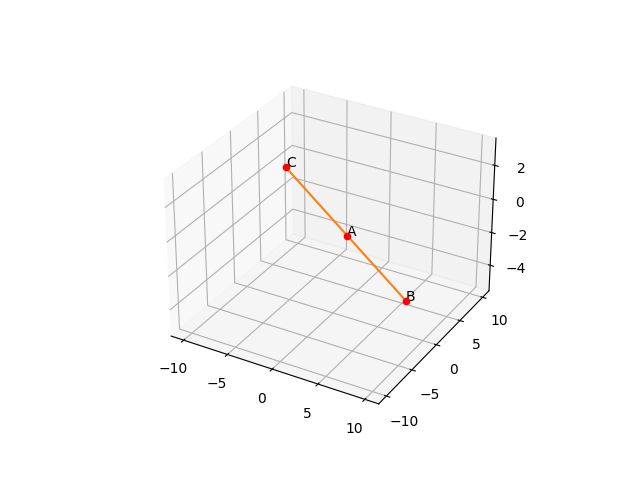
\includegraphics[width=\columnwidth]{chapters/12/11/3/6/figs/collinear_points.png}
    \caption{}
     \label{fig:chapters/12/11/3/6/1}
     \end{figure}
     \item  In this case, 
\begin{align}
\myvec{1&1&0 \\ 1&2&1 \\ -2&2&-1} \vec{n}=\vec{1}
\end{align}
\begin{align*}
\implies
\myvec{1&1&0&\vrule&1\\1&2&1&\vrule&1\\-2&2&-1&\vrule&1}
\\
\xleftrightarrow[R_3 \leftarrow R_3 + 2R_1]{R_2 \leftarrow R_2 - R_1}
\myvec{1&1&0&\vrule&1\\0&1&1&\vrule&0\\0&4&-1&\vrule&3}
\\
	\xleftrightarrow[R_3 \leftarrow R_3 - 4R_2]{R_1 \leftarrow R_1- R_2}
\myvec{1&0&-1&\vrule&1\\0&1&1&\vrule&0\\0&0&-5&\vrule&3}\\
	\xleftrightarrow[R_2 \leftarrow 5R_2 + R_3]{R_1 \leftarrow 5R_1- R_3}
\myvec{5&0&0&\vrule&2\\0&5&0&\vrule&3\\0&0&5&\vrule&-3}
\end{align*}
Hence, the equation of the plane is
\begin{align}
\myvec{2 & 3 & -3} \vec{x} = 5
\end{align}
\end{enumerate}

	\item Find the equation of the plane with an intercept 3 on the Y-axis and parallel to ZOX-Plane.\\
    \solution
		\iffalse
\documentclass[A4,12pt,twocolumn]{IEEEtran}
%
\usepackage{setspace}
\usepackage{gensymb}
%\doublespacing
\singlespacing

%\usepackage{graphicx}
%\usepackage{amssymb}
%\usepackage{relsize}
\usepackage[cmex10]{amsmath}
%\usepackage{amsthm}
%\interdisplaylinepenalty=2500
%\savesymbol{iint}
%\usepackage{txfonts}
%\restoresymbol{TXF}{iint}
%\usepackage{wasysym}
\usepackage{amsthm}
%\usepackage{iithtlc}
\usepackage{mathrsfs}
\usepackage{txfonts}
\usepackage{stfloats}
\usepackage{bm}
\usepackage{cite}
\usepackage{cases}
\usepackage{subfig}
%\usepackage{xtab}
\usepackage{longtable}
\usepackage{multirow}
%\usepackage{algorithm}
%\usepackage{algpseudocode}
\usepackage{enumitem}
\usepackage{mathtools}
\usepackage{steinmetz}
\usepackage{tikz}
\usepackage{circuitikz}
\usepackage{verbatim}
\usepackage{tfrupee}
\usepackage[breaklinks=true]{hyperref}
%\usepackage{stmaryrd}
\usepackage{tkz-euclide} % loads  TikZ and tkz-base
%\usetkzobj{all}
\usetikzlibrary{calc,math}
\usepackage{listings}
    \usepackage{color}                                            %%
    \usepackage{array}                                            %%
    \usepackage{longtable}                                        %%
    \usepackage{calc}                                             %%
    \usepackage{multirow}                                         %%
    \usepackage{hhline}                                           %%
    \usepackage{ifthen}                                           %%
  %optionally (for landscape tables embedded in another document): %%
    \usepackage{lscape}     
\usepackage{multicol}
\usepackage{chngcntr}
%\usepackage{enumerate}

%\usepackage{wasysym}
%\newcounter{MYtempeqncnt}
\DeclareMathOperator*{\Res}{Res}
%\renewcommand{\baselinestretch}{2}
\renewcommand\thesection{\arabic{section}}
\renewcommand\thesubsection{\thesection.\arabic{subsection}}
\renewcommand\thesubsubsection{\thesubsection.\arabic{subsubsection}}

\renewcommand\thesectiondis{\arabic{section}}
\renewcommand\thesubsectiondis{\thesectiondis.\arabic{subsection}}
\renewcommand\thesubsubsectiondis{\thesubsectiondis.\arabic{subsubsection}}

% correct bad hyphenation here
\hyphenation{op-tical net-works semi-conduc-tor}
\def\inputGnumericTable{}                                 %%

\lstset{
%language=C,
frame=single, 
breaklines=true,
columns=fullflexible
}
%\lstset{
%language=tex,
%frame=single, 
%breaklines=true
%}

\begin{document}
%


\newtheorem{theorem}{Theorem}[section]
\newtheorem{problem}{Problem}
\newtheorem{proposition}{Proposition}[section]
\newtheorem{lemma}{Lemma}[section]
\newtheorem{corollary}[theorem]{Corollary}
\newtheorem{example}{Example}[section]
\newtheorem{definition}[problem]{Definition}
%\newtheorem{thm}{Theorem}[section] 
%\newtheorem{defn}[thm]{Definition}
%\newtheorem{algorithm}{Algorithm}[section]
%\newtheorem{cor}{Corollary}
\newcommand{\BEQA}{\begin{eqnarray}}
\newcommand{\EEQA}{\end{eqnarray}}
\newcommand{\define}{\stackrel{\triangle}{=}}

\bibliographystyle{IEEEtran}
%\bibliographystyle{ieeetr}


\providecommand{\mbf}{\mathbf}
\providecommand{\pr}[1]{\ensuremath{\Pr\left(#1\right)}}
\providecommand{\qfunc}[1]{\ensuremath{Q\left(#1\right)}}
\providecommand{\sbrak}[1]{\ensuremath{{}\left[#1\right]}}
\providecommand{\lsbrak}[1]{\ensuremath{{}\left[#1\right.}}
\providecommand{\rsbrak}[1]{\ensuremath{{}\left.#1\right]}}
\providecommand{\brak}[1]{\ensuremath{\left(#1\right)}}
\providecommand{\lbrak}[1]{\ensuremath{\left(#1\right.}}
\providecommand{\rbrak}[1]{\ensuremath{\left.#1\right)}}
\providecommand{\cbrak}[1]{\ensuremath{\left\{#1\right\}}}
\providecommand{\lcbrak}[1]{\ensuremath{\left\{#1\right.}}
\providecommand{\rcbrak}[1]{\ensuremath{\left.#1\right\}}}
\theoremstyle{remark}
\newtheorem{rem}{Remark}
\newcommand{\sgn}{\mathop{\mathrm{sgn}}}
\providecommand{\abs}[1]{\left\vert#1\right\vert}
\providecommand{\res}[1]{\Res\displaylimits_{#1}} 
\providecommand{\norm}[1]{\left\lVert#1\right\rVert}
%\providecommand{\norm}[1]{\lVert#1\rVert}
\providecommand{\mtx}[1]{\mathbf{#1}}
\providecommand{\mean}[1]{E\left[ #1 \right]}
\providecommand{\fourier}{\overset{\mathcal{F}}{ \rightleftharpoons}}
%\providecommand{\hilbert}{\overset{\mathcal{H}}{ \rightleftharpoons}}
\providecommand{\system}{\overset{\mathcal{H}}{ \longleftrightarrow}}
	%\newcommand{\solution}[2]{\textbf{Solution:}{#1}}
\newcommand{\solution}{\noindent \textbf{Solution: }}
\newcommand{\cosec}{\,\text{cosec}\,}
\providecommand{\dec}[2]{\ensuremath{\overset{#1}{\underset{#2}{\gtrless}}}}
\newcommand{\myvec}[1]{\ensuremath{\begin{pmatrix}#1\end{pmatrix}}}
\newcommand{\mydet}[1]{\ensuremath{\begin{vmatrix}#1\end{vmatrix}}}
%\numberwithin{equation}{section}
\numberwithin{equation}{subsection}
%\numberwithin{problem}{section}
%\numberwithin{definition}{section}
\makeatletter
\@addtoreset{figure}{problem}
\makeatother

\let\StandardTheFigure\thefigure
\let\vec\mathbf
%\renewcommand{\thefigure}{\theproblem.\arabic{figure}}
\renewcommand{\thefigure}{\theproblem}
%\setlist[enumerate,1]{before=\renewcommand\theequation{\theenumi.\arabic{equation}}
%\counterwithin{equation}{enumi}


%\renewcommand{\theequation}{\arabic{subsection}.\arabic{equation}}

\def\putbox#1#2#3{\makebox[0in][l]{\makebox[#1][l]{}\raisebox{\baselineskip}[0in][0in]{\raisebox{#2}[0in][0in]{#3}}}}
     \def\rightbox#1{\makebox[0in][r]{#1}}
     \def\centbox#1{\makebox[0in]{#1}}
     \def\topbox#1{\raisebox{-\baselineskip}[0in][0in]{#1}}
     \def\midbox#1{\raisebox{-0.5\baselineskip}[0in][0in]{#1}}

\vspace{3cm}


\title{GEOMETRY}
\author{Shristy Sharma (EE22BNITS11001)}





% make the title area
\maketitle

\newpage

%\tableofcontents

\bigskip

\renewcommand{\thefigure}{\theenumi}
\renewcommand{\thetable}{\theenumi}
%\renewcommand{\theequation}{\theenumi}


%Download all python codes 
%
%\begin{lstlisting}
%svn co https://github.com/JayatiD93/trunk/My_solution_design/codes
%\end{lstlisting}

%Download all and latex-tikz codes from 
%
%\begin{lstlisting}
%svn co https://github.com/gadepall/school/trunk/ncert/geometry/figs
%\end{lstlisting}
%


\section{PROBLEM 1}
SOLUTION:\\
\fi
The normal vector to the ZOX plane is
\begin{align} 
\vec{n} = \myvec{0\\1\\0}.
\end{align}
Since, Y-axis has the intercept 3, the desired plane passes through the point
\begin{align}
\vec{P}=\myvec{0\\3\\0}.
\end{align}
Thus, the equation of the plane is given by,
\begin{align}
	\vec{n}^\top \brak{\vec{x}-\vec{P}} &= 0\\
	\implies \myvec{0&1&0} \vec{x}&= 3
\end{align}
See Fig. 
     \ref{fig:chapters/12/11/3/8/1}.
\begin{figure}[h!]
  \centering
   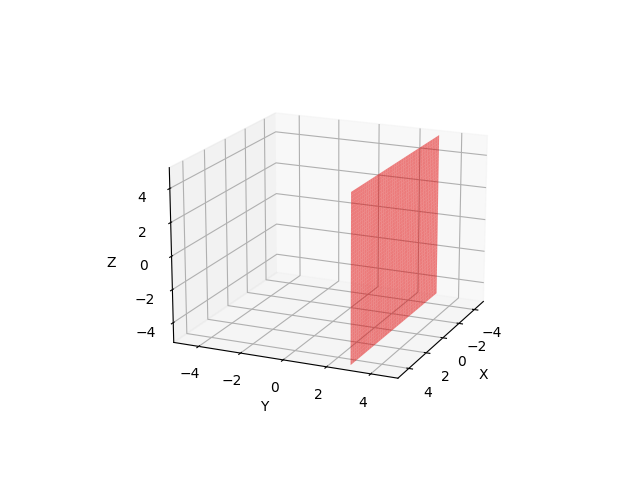
\includegraphics[width=\columnwidth]{chapters/12/11/3/8/figs/plane1.png}
    \caption{}
     \label{fig:chapters/12/11/3/8/1}
     \end{figure}  

	\item  Find the equation of the plane through the intersection of the planes $3{x} – {y} + 2{z} – 4 = 0 \text{ and } {x} + {y} + {z} – 2 = 0$ and the point $\myvec{2\\2\\1}$.
    \solution
		\iffalse
\documentclass[journal,12pt,twocolumn]{IEEEtran}
\usepackage{setspace}
\usepackage{gensymb}
\usepackage{xcolor}
\usepackage{caption}
\singlespacing
\usepackage{siunitx}
\usepackage[cmex10]{amsmath}
\usepackage{mathtools}
\usepackage{hyperref}
\usepackage{amsthm}
\usepackage{mathrsfs}
\usepackage{txfonts}
\usepackage{stfloats}
\usepackage{cite}
\usepackage{cases}
\usepackage{subfig}
\usepackage{longtable}
\usepackage{multirow}
\usepackage{enumitem}
\usepackage{bm}
\usepackage{mathtools}
\usepackage{listings}
\usepackage{tikz}
\usetikzlibrary{shapes,arrows,positioning}
\usepackage{circuitikz}
\renewcommand{\vec}[1]{\boldsymbol{\mathbf{#1}}}
\DeclareMathOperator*{\Res}{Res}
\renewcommand\thesection{\arabic{section}}
\renewcommand\thesubsection{\thesection.\arabic{subsection}}
\renewcommand\thesubsubsection{\thesubsection.\arabic{subsubsection}}

\renewcommand\thesectiondis{\arabic{section}}
\renewcommand\thesubsectiondis{\thesectiondis.\arabic{subsection}}
\renewcommand\thesubsubsectiondis{\thesubsectiondis.\arabic{subsubsection}}
\hyphenation{op-tical net-works semi-conduc-tor}

\lstset{
language=Python,
frame=single, 
breaklines=true,
columns=fullflexible
}
\begin{document}
\theoremstyle{definition}
\newtheorem{theorem}{Theorem}[section]
\newtheorem{problem}{Problem}
\newtheorem{proposition}{Proposition}[section]
\newtheorem{lemma}{Lemma}[section]
\newtheorem{corollary}[theorem]{Corollary}
\newtheorem{example}{Example}[section]
\newtheorem{definition}{Definition}[section]
\newcommand{\BEQA}{\begin{eqnarray}}
        \newcommand{\EEQA}{\end{eqnarray}}
\newcommand{\define}{\stackrel{\triangle}{=}}
\newcommand{\myvec}[1]{\ensuremath{\begin{pmatrix}#1\end{pmatrix}}}
\newcommand{\mydet}[1]{\ensuremath{\begin{vmatrix}#1\end{vmatrix}}}
\bibliographystyle{IEEEtran}
\providecommand{\nCr}[2]{\,^{#1}C_{#2}} % nCr
\providecommand{\nPr}[2]{\,^{#1}P_{#2}} % nPr
\providecommand{\mbf}{\mathbf}
\providecommand{\pr}[1]{\ensuremath{\Pr\left(#1\right)}}
\providecommand{\qfunc}[1]{\ensuremath{Q\left(#1\right)}}
\providecommand{\sbrak}[1]{\ensuremath{{}\left[#1\right]}}
\providecommand{\lsbrak}[1]{\ensuremath{{}\left[#1\right.}}
\providecommand{\rsbrak}[1]{\ensuremath{{}\left.#1\right]}}
\providecommand{\brak}[1]{\ensuremath{\left(#1\right)}}
\providecommand{\lbrak}[1]{\ensuremath{\left(#1\right.}}
\providecommand{\rbrak}[1]{\ensuremath{\left.#1\right)}}
\providecommand{\cbrak}[1]{\ensuremath{\left\{#1\right\}}}
\providecommand{\lcbrak}[1]{\ensuremath{\left\{#1\right.}}
\providecommand{\rcbrak}[1]{\ensuremath{\left.#1\right\}}}
\theoremstyle{remark}
\newtheorem{rem}{Remark}
\newcommand{\sgn}{\mathop{\mathrm{sgn}}}
\newcommand{\rect}{\mathop{\mathrm{rect}}}
\newcommand{\sinc}{\mathop{\mathrm{sinc}}}
\providecommand{\abs}[1]{\left\vert#1\right\vert}
\providecommand{\res}[1]{\Res\displaylimits_{#1}}
\providecommand{\norm}[1]{\lVert#1\rVert}
\providecommand{\mtx}[1]{\mathbf{#1}}
\providecommand{\mean}[1]{E\left[ #1 \right]}
\providecommand{\fourier}{\overset{\mathcal{F}}{ \rightleftharpoons}}
\providecommand{\ztrans}{\overset{\mathcal{Z}}{ \rightleftharpoons}}
\providecommand{\system}[1]{\overset{\mathcal{#1}}{ \longleftrightarrow}}
\newcommand{\solution}{\noindent \textbf{Solution: }}
\providecommand{\dec}[2]{\ensuremath{\overset{#1}{\underset{#2}{\gtrless}}}}
\let\StandardTheFigure\thefigure
\def\putbox#1#2#3{\makebox[0in][l]{\makebox[#1][l]{}\raisebox{\baselineskip}[0in][0in]{\raisebox{#2}[0in][0in]{#3}}}}
\def\rightbox#1{\makebox[0in][r]{#1}}
\def\centbox#1{\makebox[0in]{#1}}
\def\topbox#1{\raisebox{-\baselineskip}[0in][0in]{#1}}
\def\midbox#1{\raisebox{-0.5\baselineskip}[0in][0in]{#1}}

\vspace{3cm}
\title{12.11.3.9}
\author{Lokesh Surana}
\maketitle
\section*{Class 12, Chapter 11, Exercise 3.9}


\solution The equation of given are given by
\begin{align}
	 {P}_1: \vec{n}_1^{\top}{\vec{x}} &= {c}_1\\
	 {P}_1: \vec{n}_1^{\top}{\vec{x}} &= {c}_2
\end{align}
%
\fi
The parameters of the given planes are
\begin{align}
 \vec{n}_1 = \myvec{3\\-1\\2},\,
 \vec{n}_1 = \myvec{1\\1\\1},\,
	c_1 = 4, c_2 = 2.
\end{align}
The intersection of the planes is given as
\begin{align}
\vec{n}_1^{\top}{\vec{x}} - {c}_1 + \lambda\brak{\vec{n}_2^{\top}{\vec{x}} - {c}_2} &= 0
\end{align}
where 
\begin{align}
	\lambda = \frac{{c}_1 - {n}_1^{\top}\vec{P}}{{n}_2^{\top}\vec{P} - {c}_2} 
= -\frac{2}{3}  
\end{align}
upon substituting 
\begin{align}
\vec{P} = \myvec{2\\2\\1}
\end{align}
Thus, 
the equation of plane is 
\begin{align}
 \myvec{7&-5&4}\vec{x} = 8
\end{align}


\item 
	Find the Cartesian equation of the following planes:


\begin{enumerate}
    \item $\vec{r}.\brak{\hat{i}+\hat{j}-\hat{k}}=2$
    \item $\vec{r}.\brak{2\hat{i}+3\hat{j}-4\hat{k}}=1$
    \item $\vec{r}.[\brak{s-2t}\hat{i}+\brak{3-t}\hat{j}+\brak{2s+t}\hat{k}]=15$
\end{enumerate}


\textbf{Solution :}
\begin{enumerate}
    \item $\myvec{1&1&-1} \vec{x} = 2$
    \item $\myvec{2&3&-4} \vec{x} = 1$
    \item $\myvec{2&-5&-1} \vec{x} = 15$

\end{enumerate}




\end{enumerate}

